% Options for packages loaded elsewhere
\PassOptionsToPackage{unicode}{hyperref}
\PassOptionsToPackage{hyphens}{url}
%
\documentclass[
]{book}
\usepackage{lmodern}
\usepackage{amssymb,amsmath}
\usepackage{ifxetex,ifluatex}
\ifnum 0\ifxetex 1\fi\ifluatex 1\fi=0 % if pdftex
  \usepackage[T1]{fontenc}
  \usepackage[utf8]{inputenc}
  \usepackage{textcomp} % provide euro and other symbols
\else % if luatex or xetex
  \usepackage{unicode-math}
  \defaultfontfeatures{Scale=MatchLowercase}
  \defaultfontfeatures[\rmfamily]{Ligatures=TeX,Scale=1}
\fi
% Use upquote if available, for straight quotes in verbatim environments
\IfFileExists{upquote.sty}{\usepackage{upquote}}{}
\IfFileExists{microtype.sty}{% use microtype if available
  \usepackage[]{microtype}
  \UseMicrotypeSet[protrusion]{basicmath} % disable protrusion for tt fonts
}{}
\makeatletter
\@ifundefined{KOMAClassName}{% if non-KOMA class
  \IfFileExists{parskip.sty}{%
    \usepackage{parskip}
  }{% else
    \setlength{\parindent}{0pt}
    \setlength{\parskip}{6pt plus 2pt minus 1pt}}
}{% if KOMA class
  \KOMAoptions{parskip=half}}
\makeatother
\usepackage{xcolor}
\IfFileExists{xurl.sty}{\usepackage{xurl}}{} % add URL line breaks if available
\IfFileExists{bookmark.sty}{\usepackage{bookmark}}{\usepackage{hyperref}}
\hypersetup{
  pdftitle={A Quick Introduction to bbsBayes},
  pdfauthor={Adam C. Smith, and Brandon P.M. Edwards},
  hidelinks,
  pdfcreator={LaTeX via pandoc}}
\urlstyle{same} % disable monospaced font for URLs
\usepackage{color}
\usepackage{fancyvrb}
\newcommand{\VerbBar}{|}
\newcommand{\VERB}{\Verb[commandchars=\\\{\}]}
\DefineVerbatimEnvironment{Highlighting}{Verbatim}{commandchars=\\\{\}}
% Add ',fontsize=\small' for more characters per line
\usepackage{framed}
\definecolor{shadecolor}{RGB}{248,248,248}
\newenvironment{Shaded}{\begin{snugshade}}{\end{snugshade}}
\newcommand{\AlertTok}[1]{\textcolor[rgb]{0.94,0.16,0.16}{#1}}
\newcommand{\AnnotationTok}[1]{\textcolor[rgb]{0.56,0.35,0.01}{\textbf{\textit{#1}}}}
\newcommand{\AttributeTok}[1]{\textcolor[rgb]{0.77,0.63,0.00}{#1}}
\newcommand{\BaseNTok}[1]{\textcolor[rgb]{0.00,0.00,0.81}{#1}}
\newcommand{\BuiltInTok}[1]{#1}
\newcommand{\CharTok}[1]{\textcolor[rgb]{0.31,0.60,0.02}{#1}}
\newcommand{\CommentTok}[1]{\textcolor[rgb]{0.56,0.35,0.01}{\textit{#1}}}
\newcommand{\CommentVarTok}[1]{\textcolor[rgb]{0.56,0.35,0.01}{\textbf{\textit{#1}}}}
\newcommand{\ConstantTok}[1]{\textcolor[rgb]{0.00,0.00,0.00}{#1}}
\newcommand{\ControlFlowTok}[1]{\textcolor[rgb]{0.13,0.29,0.53}{\textbf{#1}}}
\newcommand{\DataTypeTok}[1]{\textcolor[rgb]{0.13,0.29,0.53}{#1}}
\newcommand{\DecValTok}[1]{\textcolor[rgb]{0.00,0.00,0.81}{#1}}
\newcommand{\DocumentationTok}[1]{\textcolor[rgb]{0.56,0.35,0.01}{\textbf{\textit{#1}}}}
\newcommand{\ErrorTok}[1]{\textcolor[rgb]{0.64,0.00,0.00}{\textbf{#1}}}
\newcommand{\ExtensionTok}[1]{#1}
\newcommand{\FloatTok}[1]{\textcolor[rgb]{0.00,0.00,0.81}{#1}}
\newcommand{\FunctionTok}[1]{\textcolor[rgb]{0.00,0.00,0.00}{#1}}
\newcommand{\ImportTok}[1]{#1}
\newcommand{\InformationTok}[1]{\textcolor[rgb]{0.56,0.35,0.01}{\textbf{\textit{#1}}}}
\newcommand{\KeywordTok}[1]{\textcolor[rgb]{0.13,0.29,0.53}{\textbf{#1}}}
\newcommand{\NormalTok}[1]{#1}
\newcommand{\OperatorTok}[1]{\textcolor[rgb]{0.81,0.36,0.00}{\textbf{#1}}}
\newcommand{\OtherTok}[1]{\textcolor[rgb]{0.56,0.35,0.01}{#1}}
\newcommand{\PreprocessorTok}[1]{\textcolor[rgb]{0.56,0.35,0.01}{\textit{#1}}}
\newcommand{\RegionMarkerTok}[1]{#1}
\newcommand{\SpecialCharTok}[1]{\textcolor[rgb]{0.00,0.00,0.00}{#1}}
\newcommand{\SpecialStringTok}[1]{\textcolor[rgb]{0.31,0.60,0.02}{#1}}
\newcommand{\StringTok}[1]{\textcolor[rgb]{0.31,0.60,0.02}{#1}}
\newcommand{\VariableTok}[1]{\textcolor[rgb]{0.00,0.00,0.00}{#1}}
\newcommand{\VerbatimStringTok}[1]{\textcolor[rgb]{0.31,0.60,0.02}{#1}}
\newcommand{\WarningTok}[1]{\textcolor[rgb]{0.56,0.35,0.01}{\textbf{\textit{#1}}}}
\usepackage{longtable,booktabs}
% Correct order of tables after \paragraph or \subparagraph
\usepackage{etoolbox}
\makeatletter
\patchcmd\longtable{\par}{\if@noskipsec\mbox{}\fi\par}{}{}
\makeatother
% Allow footnotes in longtable head/foot
\IfFileExists{footnotehyper.sty}{\usepackage{footnotehyper}}{\usepackage{footnote}}
\makesavenoteenv{longtable}
\usepackage{graphicx}
\makeatletter
\def\maxwidth{\ifdim\Gin@nat@width>\linewidth\linewidth\else\Gin@nat@width\fi}
\def\maxheight{\ifdim\Gin@nat@height>\textheight\textheight\else\Gin@nat@height\fi}
\makeatother
% Scale images if necessary, so that they will not overflow the page
% margins by default, and it is still possible to overwrite the defaults
% using explicit options in \includegraphics[width, height, ...]{}
\setkeys{Gin}{width=\maxwidth,height=\maxheight,keepaspectratio}
% Set default figure placement to htbp
\makeatletter
\def\fps@figure{htbp}
\makeatother
\setlength{\emergencystretch}{3em} % prevent overfull lines
\providecommand{\tightlist}{%
  \setlength{\itemsep}{0pt}\setlength{\parskip}{0pt}}
\setcounter{secnumdepth}{5}
\ifluatex
  \usepackage{selnolig}  % disable illegal ligatures
\fi
\newlength{\cslhangindent}
\setlength{\cslhangindent}{1.5em}
\newlength{\csllabelwidth}
\setlength{\csllabelwidth}{3em}
\newenvironment{CSLReferences}[3] % #1 hanging-ident, #2 entry sp
 {% don't indent paragraphs
  \setlength{\parindent}{0pt}
  % turn on hanging indent if param 1 is 1
  \ifodd #1 \everypar{\setlength{\hangindent}{\cslhangindent}}\ignorespaces\fi
  % set line spacing
  % set entry spacing
  \ifnum #2 > 0
  \setlength{\parskip}{#3\baselineskip}
  \fi
 }%
 {}
\usepackage{calc} % for \widthof, \maxof
\newcommand{\CSLBlock}[1]{#1\hfill\break}
\newcommand{\CSLLeftMargin}[1]{\parbox[t]{\maxof{\widthof{#1}}{\csllabelwidth}}{#1}}
\newcommand{\CSLRightInline}[1]{\parbox[t]{\linewidth}{#1}}
\newcommand{\CSLIndent}[1]{\hspace{\cslhangindent}#1}

\title{A Quick Introduction to bbsBayes}
\author{Adam C. Smith, and Brandon P.M. Edwards}
\date{2020-12-14}

\begin{document}
\maketitle

{
\setcounter{tocdepth}{1}
\tableofcontents
}
\hypertarget{customized-bbs-trends-trajectories-graphs-and-maps-using-the-bbsbayes-r-package-an-introduction}{%
\chapter{Customized BBS trends, trajectories, graphs, and maps using the bbsBayes R-package, an Introduction}\label{customized-bbs-trends-trajectories-graphs-and-maps-using-the-bbsbayes-r-package-an-introduction}}

\hypertarget{what-is-the-workshop-about}{%
\section{What is the workshop about?}\label{what-is-the-workshop-about}}

This is a 2-hour introductory workshop/demonstration of the R-package
bbsBayes (\url{https://github.com/BrandonEdwards/bbsBayes}). This package
allows anyone to apply the hierarchical Bayesian models used to estimate
status and trends from the North American Breeding Bird Survey. The
package also lets the user generate a suite of alternative metrics using
the existing model output from the annual CWS analyses.

\hypertarget{intended-audience}{%
\section{Intended Audience}\label{intended-audience}}

Everyone is welcome! Some familiarity working with R is required if
you'd also like to run the code yourself during the workshop, and the
relevant packages should be installed beforehand (details will be
provided with a full outline to be provided closer to the date). Those
who might particularly be interested in attending include:

\begin{enumerate}
\def\labelenumi{\arabic{enumi}.}
\item
  Anyone who might wish for a BBS trend for a particular region or
  time-period (e.g,. I want 15-year trends not 10-year trends, I wish
  I had a trend for just the western portion of the Barn Swallow's
  range),
\item
  Anyone who might want to analyse the BBS with a customized model
  (e.g., the effect of weather, land-cover, etc. on trends). Do not
  worry if Bayesian analyses are new to you. We will not review the
  basics of Bayesian statistical analyses, but the package can be very
  useful without understanding those basics.
\end{enumerate}

\hypertarget{what-we-hope-you-will-learn-here}{%
\section{What we hope you will learn here}\label{what-we-hope-you-will-learn-here}}

\begin{itemize}
\item
  Download the raw data
\item
  Choose and run a model, geographic stratification, and species (we
  will not cover formal model-selection, just explore the different
  model-options)
\item
  Estimate trends for any time-period (1970-2019, 2005-2015,
  1980-2000, etc.)
\item
  Graph population trajectories
\item
  Generate heat maps of population trends
\item
  Create geofaceted trajectory plots
\item
  Estimate trends for customized regions (e.g., All of the eastern
  Boreal, Great Plains vs eastern populations of grassland birds)
\end{itemize}

\hypertarget{Intro}{%
\chapter{Preparation and Installation}\label{Intro}}

\hypertarget{pre-workshop-preparation}{%
\section{Pre-Workshop preparation}\label{pre-workshop-preparation}}

We will present this initial workshop primarily as a demonstration. So you do not need to run any actual code, in order to get a good sense of what the package can do.

If you are reasonably familiar with using R, and you do want to follow along with the coding during the workshop, please ensure you have installed the most recent version of R (4.0.3) and RStudio.

In addition, please install the bbsBayes package and download the data.

Finally, if you haven't used JAGS before, you'll also need to install this stand-alone program (the Bayesian MCMC software that the package relies on). Follow the link below to download the installer.

\hypertarget{installation}{%
\section{Installation}\label{installation}}

bbsBayes is on CRAN! There are two ways to install the package:

Option 1: Stable release from CRAN

\begin{Shaded}
\begin{Highlighting}[]
\CommentTok{\# To install from CRAN:}
\FunctionTok{install.packages}\NormalTok{(}\StringTok{"bbsBayes"}\NormalTok{)}
\end{Highlighting}
\end{Shaded}

Option 2: Less-stable development version

\begin{Shaded}
\begin{Highlighting}[]
\CommentTok{\# To install the development version from GitHub:}
\FunctionTok{install.packages}\NormalTok{(}\StringTok{"devtools"}\NormalTok{)}
\FunctionTok{library}\NormalTok{(devtools)}
\NormalTok{devtools}\SpecialCharTok{::}\FunctionTok{install\_github}\NormalTok{(}\StringTok{"BrandonEdwards/bbsBayes"}\NormalTok{)}
\end{Highlighting}
\end{Shaded}

\hypertarget{data-retrieval}{%
\section{Data Retrieval}\label{data-retrieval}}

You can download BBS data by running \texttt{fetch\_bbs\_data}. This will save the data to a package-specific directory on your computer. You must agree to the terms and conditions of the data usage before the download will run {[}type yes at the prompt{]}. You only need run this function once for each annual update of the BBS database.

\begin{Shaded}
\begin{Highlighting}[]
\FunctionTok{fetch\_bbs\_data}\NormalTok{()}
\end{Highlighting}
\end{Shaded}

There are options to download the available stop-level data, so you can use the package to access these data. However, for now the bbsBayes modeling functions only work with the route-level summaries. So use the defaults in the function.

\hypertarget{install-jags}{%
\section{Install JAGS}\label{install-jags}}

The modeling functions of bbsBayes require an installation of JAGS. JAGS is installed from SourceForge, an open software distribution agent. Follow \href{https://sourceforge.net/projects/mcmc-jags/}{this link} to install {[}\url{https://sourceforge.net/projects/mcmc-jags/}{]}.

\hypertarget{example-data-for-scarlet-tanager}{%
\section{Example data for Scarlet Tanager}\label{example-data-for-scarlet-tanager}}

This \href{https://drive.google.com/file/d/1LCZrl0W0AEbXj8_MyUP-CXX3a-j77rFN/view?usp=sharing}{link allows you to download some example model results for Scarlet Tanager}. This model output can be used with many of the visualization and estimation functions for the package (without having to wait \textasciitilde24 hours for the model to run). To use this saved results to run some of the functions in this book, save it into your working directory.

\hypertarget{Stratify}{%
\chapter{Stratification}\label{Stratify}}

\hypertarget{strata}{%
\section{Strata}\label{strata}}

All of the models supported by bbsBayes expect the BBS route-level data to be grouped into geographic strata. These strata are subregions of the survey area, and allow the parameters that model abundance and trend to vary across a species' range.

Use the \texttt{stratify()} function to group the BBS data into one of the included stratifications. Select the stratification using the argument \texttt{by} to stratify by the following options:

\begin{itemize}
\tightlist
\item
  bbs\_cws -- \texttt{stratify(by\ =\ "bbs\_cws")} Political region X Bird Conservation region intersection (Canadian Wildlife Service {[}CWS{]} method). Identical to bbs\_usgs, except all routes in BCR 7 are combined into a single stratum, and all routes in PEI and Nova Scotia are combined into a single stratum.
\end{itemize}

\begin{itemize}
\tightlist
\item
  bbs\_usgs -- \texttt{stratify(by\ =\ "bbs\_usgs")} Political region X Bird Conservation region intersection (United Status Geological Survey {[}USGS{]} method)
\end{itemize}

\begin{itemize}
\tightlist
\item
  bcr -- \texttt{stratify(by\ =\ "bcr")} Bird Conservation Region only
\end{itemize}

\begin{itemize}
\tightlist
\item
  state -- \texttt{stratify(by\ =\ "state")} Political Region only
\end{itemize}

\begin{itemize}
\tightlist
\item
  latlong -- \texttt{stratify(by\ =\ "latlong")} Degree blocks (1 degree of latitude X 1 degree of longitude)
\end{itemize}

Now that we know the built-in stratification options, let's stratify our copy of the BBS data. Here, we will choose to stratify our data using the ``bbs\_cws'' method:

\begin{Shaded}
\begin{Highlighting}[]
\CommentTok{\# set up for the annual CWS status and trend analysis}
\NormalTok{strat\_data }\OtherTok{\textless{}{-}} \FunctionTok{stratify}\NormalTok{(}\AttributeTok{by =} \StringTok{"bbs\_cws"}\NormalTok{)}
\end{Highlighting}
\end{Shaded}

The stratified\_data object includes 3 dataframes.

\begin{itemize}
\tightlist
\item
  \texttt{strat\_data\$species\_strat} is a table of all species included in the dataset. It has columns for species common names in English, French, and Spanish, as well as information on the order, family, genus, species, and the numerical species indicators used in the BBS database in both character format (with leading 0s) and integer format.
\end{itemize}

\begin{Shaded}
\begin{Highlighting}[]
\NormalTok{knitr}\SpecialCharTok{::}\FunctionTok{kable}\NormalTok{(}\FunctionTok{head}\NormalTok{(strat\_data}\SpecialCharTok{$}\NormalTok{species\_strat[,}\FunctionTok{c}\NormalTok{(}\DecValTok{3}\NormalTok{,}\DecValTok{4}\NormalTok{,}\DecValTok{5}\NormalTok{,}\DecValTok{8}\NormalTok{,}\DecValTok{9}\NormalTok{,}\DecValTok{10}\NormalTok{)]))}
\end{Highlighting}
\end{Shaded}

\begin{tabular}{l|l|l|l|l|r}
\hline
english & french & spanish & genus & species & sp.bbs\\
\hline
Black-bellied Whistling-Duck & Dendrocygne à ventre noir & Dendrocygna autumnalis & Dendrocygna & autumnalis & 1770\\
\hline
Fulvous Whistling-Duck & Dendrocygne fauve & Dendrocygna bicolor & Dendrocygna & bicolor & 1780\\
\hline
Emperor Goose & Oie empereur & Anser canagicus & Anser & canagicus & 1760\\
\hline
Snow Goose (all forms) & Oie des neiges (toutes les formes) & Anser caerulescens & Anser & caerulescens & 1690\\
\hline
(Blue Goose) Snow Goose & Oie des neiges (forme bleue) & Anser caerulescens (blue form) & Anser & caerulescens (blue form) & 1691\\
\hline
Ross's Goose & Oie de Ross & Anser rossii & Anser & rossii & 1700\\
\hline
\end{tabular}

\begin{itemize}
\tightlist
\item
  \texttt{strat\_data\$bird\_strat} is a very large table of each observed count for a given species X route X year combination. This is the table that includes all of the non-zero observations in the BBS database.
\end{itemize}

\begin{Shaded}
\begin{Highlighting}[]
\NormalTok{knitr}\SpecialCharTok{::}\FunctionTok{kable}\NormalTok{(}\FunctionTok{head}\NormalTok{(strat\_data}\SpecialCharTok{$}\NormalTok{bird\_strat[,}\FunctionTok{c}\NormalTok{(}\DecValTok{1}\NormalTok{,}\DecValTok{2}\NormalTok{,}\DecValTok{6}\NormalTok{,}\DecValTok{7}\NormalTok{,}\DecValTok{14}\NormalTok{,}\DecValTok{16}\NormalTok{,}\DecValTok{17}\NormalTok{)]))}
\end{Highlighting}
\end{Shaded}

\begin{tabular}{r|r|r|r|r|l|l}
\hline
statenum & Route & Year & AOU & SpeciesTotal & rt.uni & rt.uni.y\\
\hline
11 & 1 & 1997 & 5880 & 28 & 11-1 & 11-1-1997\\
\hline
11 & 1 & 1997 & 5671 & 6 & 11-1 & 11-1-1997\\
\hline
11 & 1 & 1997 & 6850 & 3 & 11-1 & 11-1-1997\\
\hline
11 & 1 & 1991 & 6882 & 22 & 11-1 & 11-1-1991\\
\hline
11 & 1 & 2012 & 3160 & 1 & 11-1 & 11-1-2012\\
\hline
11 & 1 & 1991 & 4860 & 9 & 11-1 & 11-1-1991\\
\hline
\end{tabular}

\begin{itemize}
\tightlist
\item
  \texttt{strat\_data\$route\_strat} is a large table of each BBS survey conducted. It includes a single row for each survey-event (i.e., a route X year X observer combination). It also includes the information on the weather conditions, timing, date, etc.
\end{itemize}

\begin{Shaded}
\begin{Highlighting}[]
\NormalTok{knitr}\SpecialCharTok{::}\FunctionTok{kable}\NormalTok{(}\FunctionTok{head}\NormalTok{(strat\_data}\SpecialCharTok{$}\NormalTok{route\_strat[,}\FunctionTok{c}\NormalTok{(}\DecValTok{2}\NormalTok{,}\DecValTok{3}\NormalTok{,}\DecValTok{8}\NormalTok{,}\DecValTok{13}\NormalTok{,}\DecValTok{33}\SpecialCharTok{:}\DecValTok{35}\NormalTok{)]))}
\end{Highlighting}
\end{Shaded}

\begin{tabular}{r|r|r|r|l|l|l}
\hline
statenum & Route & BCR & Year & strat\_name & rt.uni & rt.uni.y\\
\hline
11 & 1 & 5 & 1995 & CA-BC-5 & 11-1 & 11-1-1995\\
\hline
11 & 1 & 5 & 1994 & CA-BC-5 & 11-1 & 11-1-1994\\
\hline
11 & 1 & 5 & 1976 & CA-BC-5 & 11-1 & 11-1-1976\\
\hline
11 & 1 & 5 & 1977 & CA-BC-5 & 11-1 & 11-1-1977\\
\hline
11 & 1 & 5 & 1974 & CA-BC-5 & 11-1 & 11-1-1974\\
\hline
11 & 1 & 5 & 1975 & CA-BC-5 & 11-1 & 11-1-1975\\
\hline
\end{tabular}

\hypertarget{useful-code-to-access-and-print-the-strata-maps-above}{%
\subsection{Useful code to access and print the strata maps above}\label{useful-code-to-access-and-print-the-strata-maps-above}}

The package does not include functions to directly access the strata maps (other than the \texttt{generate\_map()} function, which displays a map of estimated trends). However this code below should suffice to find the map files in your local installation.

\begin{Shaded}
\begin{Highlighting}[]
\FunctionTok{library}\NormalTok{(sf)}
\FunctionTok{library}\NormalTok{(sp)}
\FunctionTok{library}\NormalTok{(ggplot2)}
\NormalTok{laea }\OtherTok{=} \FunctionTok{st\_crs}\NormalTok{(}\StringTok{"+proj=laea +lat\_0=40 +lon\_0={-}95"}\NormalTok{) }\CommentTok{\# Lambert equal area coord reference system}

\NormalTok{strat\_maps }\OtherTok{\textless{}{-}} \FunctionTok{c}\NormalTok{(}\StringTok{"BBS\_CWS\_strata"}\NormalTok{,}
\StringTok{"BBS\_USGS\_strata"}\NormalTok{,}
\StringTok{"BBS\_BCR\_strata"}\NormalTok{,}
\StringTok{"BBS\_LatLong\_strata"}\NormalTok{,}
\StringTok{"BBS\_ProvState\_strata"}\NormalTok{)}

\FunctionTok{names}\NormalTok{(strat\_maps) }\OtherTok{\textless{}{-}} \FunctionTok{c}\NormalTok{(}\StringTok{"bbs\_cws"}\NormalTok{,}\StringTok{"bbs\_usgs"}\NormalTok{,}\StringTok{"bcr"}\NormalTok{,}\StringTok{"latlong"}\NormalTok{,}\StringTok{"state"}\NormalTok{)}

\NormalTok{locat }\OtherTok{=} \FunctionTok{system.file}\NormalTok{(}\StringTok{"maps"}\NormalTok{,}
                    \AttributeTok{package =} \StringTok{"bbsBayes"}\NormalTok{)}

\ControlFlowTok{for}\NormalTok{(i }\ControlFlowTok{in} \DecValTok{1}\SpecialCharTok{:}\FunctionTok{length}\NormalTok{(strat\_maps))\{}
\NormalTok{  map.file }\OtherTok{=}\NormalTok{ strat\_maps[i]}
\NormalTok{  st\_nm }\OtherTok{=} \FunctionTok{names}\NormalTok{(strat\_maps)[i]}
\NormalTok{strata\_map }\OtherTok{=} \FunctionTok{read\_sf}\NormalTok{(}\AttributeTok{dsn =}\NormalTok{ locat,}
                     \AttributeTok{layer =}\NormalTok{ map.file)}
\NormalTok{strata\_map }\OtherTok{=} \FunctionTok{st\_transform}\NormalTok{(strata\_map,}\AttributeTok{crs =}\NormalTok{ laea)}
\NormalTok{st\_gg }\OtherTok{=} \FunctionTok{ggplot}\NormalTok{(}\AttributeTok{data =}\NormalTok{ strata\_map)}\SpecialCharTok{+}
\FunctionTok{geom\_sf}\NormalTok{()}\SpecialCharTok{+}
\FunctionTok{labs}\NormalTok{(}\AttributeTok{title =} \FunctionTok{paste}\NormalTok{(}\StringTok{"stratify(by ="}\NormalTok{,st\_nm,}\StringTok{")"}\NormalTok{))}



\FunctionTok{png}\NormalTok{(}\FunctionTok{paste0}\NormalTok{(}\StringTok{"images/map\_"}\NormalTok{,st\_nm,}\StringTok{".png"}\NormalTok{))}
\FunctionTok{print}\NormalTok{(st\_gg)}
\FunctionTok{dev.off}\NormalTok{()}
\NormalTok{\}}
\end{Highlighting}
\end{Shaded}

\hypertarget{DataPrep}{%
\chapter{Prepare the data for a model and species}\label{DataPrep}}

\hypertarget{prepare-data}{%
\section{Prepare data}\label{prepare-data}}

The \texttt{prepare\_jags\_data()} function is used to select a species, a model, the time-scale, etc.

The critical arguments are:

\begin{itemize}
\tightlist
\item
  strat\_data: the list of stratified data returned by \texttt{stratify()}
\item
  species\_to\_run: the English name for the species. This is currently case sensitive, and must exactly match one of the names in the english column of the species\_strat object of strat\_data i.e., \texttt{strat\_data\$species\_strat\$english}
  If you'd like to export a full list of the available species, this code will work:
\end{itemize}

\begin{Shaded}
\begin{Highlighting}[]
\FunctionTok{write.csv}\NormalTok{(strat\_data}\SpecialCharTok{$}\NormalTok{species\_strat,}\StringTok{"Full\_BBS\_speciesList.csv"}\NormalTok{)}
\end{Highlighting}
\end{Shaded}

Also, if you'd like to select a species using the French name, you can try this approach:

\begin{Shaded}
\begin{Highlighting}[]
\NormalTok{espece }\OtherTok{=} \StringTok{"Colibri à gorge rubis"}
\NormalTok{species }\OtherTok{=}\NormalTok{ strat\_data}\SpecialCharTok{$}\NormalTok{species\_strat}\SpecialCharTok{$}\NormalTok{english[}\FunctionTok{which}\NormalTok{(strat\_data}\SpecialCharTok{$}\NormalTok{species\_strat}\SpecialCharTok{$}\NormalTok{french }\SpecialCharTok{==}\NormalTok{ espece)]}
\NormalTok{species}
\CommentTok{\#\textgreater{} [1] "Ruby{-}throated Hummingbird"}
\end{Highlighting}
\end{Shaded}

\begin{itemize}
\tightlist
\item
  model: the model to use, options are ``slope,'' ``firstdiff,'' ``gam,'' or ``gamye''
\end{itemize}

There are additional, optional arguments:

\begin{itemize}
\item
  heavy\_tailed - Logical indicating whether the extra-Poisson error distribution should be modeled as a t-distribution, with heavier tails than the standard normal distribution. Default is currently FALSE, but recent research suggest users should strongly consider setting this to TRUE, even though it requires much longer convergence times
\item
  n\_knots - Number of knots to be used in GAM function
\item
  min\_year - Minimum year to keep in analysis
\item
  max\_year - Maximum year to keep in analysis
\item
  min\_n\_routes - Minimum routes per strata where species has been observed. Defaults to 3, but consider lowering to 1 if using the ``latlong'' stratification
\item
  min\_max\_route\_years - Minimum number of years with non-zero observations of species on at least 1 route. Defaults to 3
\item
  min\_mean\_route\_years - Minimum average of years per route with the species observed. Defaults to 1.
\end{itemize}

\hypertarget{models}{%
\section{Models}\label{models}}

The package has (currently) four status and trend models that differ in the way they model the time-series of observations. The four model options are slope, gam, gamye, and firstdiff.

\hypertarget{slope}{%
\subsection{slope}\label{slope}}

The slope option estimates the time series as a log-linear regression with random year-effect terms that allow the trajectory to depart from the smooth regression line. It is the model used by the USGS and CWS to estimate BBS trends between 2011 and 2018. The basic model was first described in 2002 (\protect\hyperlink{ref-link2002}{Link and Sauer 2002a}) and its application to the annual status and trend estimates is documented in (\protect\hyperlink{ref-sauer2011}{Sauer and Link 2011}) and (\protect\hyperlink{ref-smith2014}{Smith et al. 2014}).

\hypertarget{gam}{%
\subsection{gam}\label{gam}}

The gam option models the time series as a semiparametric smooth using a Generalized Additive Model (GAM) structure that shares information among the strata on the shape of the population trajectory. This model is described in (\protect\hyperlink{ref-smith2020a}{Smith and Edwards 2020}).

\hypertarget{gamye}{%
\subsection{gamye}\label{gamye}}

The gamye option includes the semiparametric smooth used in the gam option, but also includes random year-effect terms that track annual fluctuations around the smooth, also in (\protect\hyperlink{ref-smith2020a}{Smith and Edwards 2020}). This is the model that the Canadian Wildlife Service is now using for the annual status and trend estimates.

\hypertarget{firstdiff}{%
\subsection{firstdiff}\label{firstdiff}}

The firstdiff option models the time-series as a random-walk from the first year, so that the first-differences of the sequence of year-effects are random effects with mean = 0 and an estimated variance. This model has been described in (\protect\hyperlink{ref-link}{Link, Sauer, and Niven, n.d.}). The first difference model is unique among these four in that it does not share information across the strata on the rate of population change. The population trajectories in each stratum are estimated independently of all other strata.

\hypertarget{cws-analysis-example}{%
\section{CWS analysis example}\label{cws-analysis-example}}

The annual CWS analysis uses the heavy-tailed version of the GAMYE model. Here's the data function call that is used in the 2019 analysis for Scarlet Tanager:

\begin{Shaded}
\begin{Highlighting}[]
\NormalTok{jags\_data }\OtherTok{\textless{}{-}} \FunctionTok{prepare\_jags\_data}\NormalTok{(}\AttributeTok{strat\_data =}\NormalTok{ strat\_data,}
                  \AttributeTok{species\_to\_run =} \StringTok{"Scarlet Tanager"}\NormalTok{,}
                  \AttributeTok{model =} \StringTok{"gamye"}\NormalTok{,}
                  \AttributeTok{min\_max\_route\_years =} \DecValTok{2}\NormalTok{,}
                  \AttributeTok{heavy\_tailed =} \ConstantTok{TRUE}\NormalTok{)}
\end{Highlighting}
\end{Shaded}

\hypertarget{ModelRun}{%
\chapter{Running the model}\label{ModelRun}}

After stratifying and preparing the data for a particular species and model, the \texttt{run\_model()} function calls the JAGS program to fit the selected model to the species' data.

Depending on the model and the size of the dataset (number of counts, number of strata, number of years, etc.), this process can take a long time (hours - days). The following code shows the settings used for most species in the annual CWS analysis.

\begin{Shaded}
\begin{Highlighting}[]
\CommentTok{\# Not Run}
\NormalTok{jags\_mod }\OtherTok{\textless{}{-}} \FunctionTok{run\_model}\NormalTok{(}\AttributeTok{jags\_data =}\NormalTok{ jags\_data,}
                      \AttributeTok{n\_iter =} \DecValTok{24000}\NormalTok{, }\CommentTok{\#higher than the default 10,000}
                      \AttributeTok{n\_burnin =} \DecValTok{20000}\NormalTok{,}
                      \AttributeTok{n\_chains =} \DecValTok{3}\NormalTok{,}
                      \AttributeTok{n\_thin =} \DecValTok{20}\NormalTok{, }\CommentTok{\#saves memory by retaining only 1/20 posterior samples}
                      \AttributeTok{parallel =} \ConstantTok{TRUE}\NormalTok{,}
                      \AttributeTok{inits =} \ConstantTok{NULL}\NormalTok{,}
                      \AttributeTok{parameters\_to\_save =} \FunctionTok{c}\NormalTok{(}\StringTok{"n"}\NormalTok{,}\StringTok{"n3"}\NormalTok{,}\StringTok{"nu"}\NormalTok{,}
                                             \StringTok{"B.X"}\NormalTok{,}\StringTok{"beta.X"}\NormalTok{,}\StringTok{"strata"}\NormalTok{,}
                                             \StringTok{"sdbeta"}\NormalTok{,}\StringTok{"sdX"}\NormalTok{,}\StringTok{"alpha"}\NormalTok{))}
 
\end{Highlighting}
\end{Shaded}

There is only one critical argument in the \texttt{run\_model()} function.

\begin{itemize}
\tightlist
\item
  jags\_data - List output from the \texttt{prepare\_jags\_data()} function.
\end{itemize}

The remaining arguments allow for some customization of the MCMC process. The default settings are sufficient for many species and model combinations, but here is some explanation of the arguments that many users may want to modify:

\begin{itemize}
\item
  parameters\_to\_save - Character vector of parameters to monitor in JAGS. Defaults to just monitoring ``n,'' the annual indices of abundance that make up the estimated population trajectories in each stratum. In the two models with separate parameters for the year-effects and the long-term change (``gamye'' and ``slope''), there is an optional version of the annual indices of abundance called ``n3,'' which tracks the population trajectory after removing the year-effects. This ``n3'' parameter represents the smooth-only population trajectory from the gamye and the linear-slope component of the trajectory from the slope model. In the CWS annual analyses, the ``n3'' parameter is used to estimate trends and the ``n'' parameter is used to track the full population trajectory.
\item
  n\_chains - Optional number of chains to run. Defaults to 3.
\item
  n\_burnin - Optional integer specifying the number of iterations to burn in the model. Defaults to 20000 per chain.
\item
  n\_thin - Optional number of steps to thin or discard. Defaults to 10
\item
  n\_iter - Optional number of iterations per chain. Defaults to 10000.
\item
  parallel - Logical, Should each chain be run in parallel on separate cores? If TRUE, the number of cores used will be the minimum of the n\_chains specified and the number of cores on your computer
\end{itemize}

\hypertarget{pacfic-wren-example}{%
\section{Pacfic Wren example}\label{pacfic-wren-example}}

Here's a toy example using data for the Pacific Wren and the slope model for a shortened time-series:

\begin{Shaded}
\begin{Highlighting}[]
\CommentTok{\#strat\_data \textless{}{-} stratify(by = "bbs\_cws")}

\CommentTok{\# Prepare the stratified data for use in a JAGS model (see Chapter 4).}
\NormalTok{jags\_data }\OtherTok{\textless{}{-}} \FunctionTok{prepare\_jags\_data}\NormalTok{(}\AttributeTok{strat\_data =}\NormalTok{ strat\_data,}
                               \AttributeTok{species\_to\_run =} \StringTok{"Pacific Wren"}\NormalTok{,}
                               \AttributeTok{model =} \StringTok{"slope"}\NormalTok{,}
                               \AttributeTok{min\_year =} \DecValTok{2009}\NormalTok{,}
                               \AttributeTok{max\_year =} \DecValTok{2018}\NormalTok{)}

\CommentTok{\# Now run the model}
\NormalTok{jags\_mod }\OtherTok{\textless{}{-}} \FunctionTok{run\_model}\NormalTok{(}\AttributeTok{jags\_data =}\NormalTok{ jags\_data,}
                      \AttributeTok{n\_adapt =} \DecValTok{100}\NormalTok{,}
                      \AttributeTok{n\_burnin =} \DecValTok{200}\NormalTok{,}
                      \AttributeTok{n\_iter =} \DecValTok{200}\NormalTok{,}
                      \AttributeTok{n\_thin =} \DecValTok{1}\NormalTok{,}
                      \AttributeTok{parameters\_to\_save =} \FunctionTok{c}\NormalTok{(}\StringTok{"n"}\NormalTok{,}\StringTok{"beta"}\NormalTok{,}\StringTok{"strata"}\NormalTok{))}
\end{Highlighting}
\end{Shaded}

\hypertarget{convergence-of-the-mcmc}{%
\section{Convergence of the MCMC}\label{convergence-of-the-mcmc}}

The \texttt{run\_model()} function will send a warning if Gelman-Rubin Rhat cross-chain convergence criterion is \textgreater{} 1.1 for any of the monitored parameters. Re-running the model with a longer burn-in and/or more posterior iterations or greater thinning rates may improve convergence. We can check for ourselves the effective sample size for each monitored parameter, as well as the Rhat values for each monitored parameter:

\begin{Shaded}
\begin{Highlighting}[]
\NormalTok{jags\_mod}\SpecialCharTok{$}\NormalTok{n.eff }\CommentTok{\#shows the effective sample size for each monitored parameter}
\NormalTok{jags\_mod}\SpecialCharTok{$}\NormalTok{Rhat }\CommentTok{\# shows the Rhat values for each monitored parameter}
\end{Highlighting}
\end{Shaded}

The seriousness of these convergence failures is something the user must interpret for themselves. In some cases some parameters of the model may not be separately estimable, but if there is no direct inference drawn from those separate parameters, their convergence may not be necessary. If all or the vast majority of the n parameters have converged (e.g., you're receiving this warning message for other monitored parameters), then inference on population trajectories and trends from the model are reliable.

If important monitored parameters have not converged, the shinystan package has some wonderful interactive tools for better understanding convergence issues with MCMC output.

\begin{Shaded}
\begin{Highlighting}[]
\CommentTok{\#install.packages("shinystan")}
\FunctionTok{library}\NormalTok{(shinystan)}
\NormalTok{my\_sso }\OtherTok{\textless{}{-}}\NormalTok{ shinystan}\SpecialCharTok{::}\FunctionTok{launch\_shinystan}\NormalTok{(shinystan}\SpecialCharTok{::}\FunctionTok{as.shinystan}\NormalTok{(jags\_mod}\SpecialCharTok{$}\NormalTok{samples, }\AttributeTok{model\_name =} \StringTok{"my\_toy\_example"}\NormalTok{))}
\end{Highlighting}
\end{Shaded}

bbsBayes also includes a function to help re-start an MCMC chain, so that you avoid having to wait for an additional burn-in period.

\begin{Shaded}
\begin{Highlighting}[]
\DocumentationTok{\#\#\# if jags\_mod has failed to converge...}
\NormalTok{new\_initials }\OtherTok{\textless{}{-}} \FunctionTok{get\_final\_values}\NormalTok{(jags\_mod)}

\NormalTok{jags\_mod2 }\OtherTok{\textless{}{-}} \FunctionTok{run\_model}\NormalTok{(}\AttributeTok{jags\_data =}\NormalTok{ jags\_data,}
                      \AttributeTok{n\_adapt =} \DecValTok{0}\NormalTok{,}
                      \AttributeTok{n\_burnin =} \DecValTok{0}\NormalTok{,}
                      \AttributeTok{n\_iter =} \DecValTok{200}\NormalTok{,}
                      \AttributeTok{n\_thin =} \DecValTok{1}\NormalTok{,}
                      \AttributeTok{inits =}\NormalTok{ new\_initials,}
                      \AttributeTok{parameters\_to\_save =} \FunctionTok{c}\NormalTok{(}\StringTok{"n"}\NormalTok{,}\StringTok{"beta"}\NormalTok{,}\StringTok{"strata"}\NormalTok{))}
\end{Highlighting}
\end{Shaded}

\hypertarget{IndicesTrends}{%
\chapter{Estimating Annual Indices and Trends}\label{IndicesTrends}}

Once the model has finished running, we can use the saved output to calculate the population trajectories and trends. As an example, we'll load some saved model output for Scarlet Tanager, from the gamye model. If you haven't already, you can download the model output file \href{https://drive.google.com/file/d/1LCZrl0W0AEbXj8_MyUP-CXX3a-j77rFN/view?usp=sharing}{here}, then save it into your working directory.

This saved workspace includes two objects:

\begin{enumerate}
\def\labelenumi{\arabic{enumi}.}
\item
  jags\_data - the data object created with the \texttt{prepare\_jags\_data()} function.
\item
  jags\_mod - the model output created with the \texttt{run\_model()} function.
\end{enumerate}

\begin{Shaded}
\begin{Highlighting}[]
\FunctionTok{load}\NormalTok{(}\StringTok{"jags\_mod\_full.RData"}\NormalTok{)}
\end{Highlighting}
\end{Shaded}

\hypertarget{annual-indices}{%
\section{Annual Indices}\label{annual-indices}}

The annual indices of relative abundance (``annual indices'') from all of the bbsBayes models represent the expected mean count on the BBS routes in a given region and year. The time-series of these annual indices in a given region make up the estimated population trajectory.

\begin{Shaded}
\begin{Highlighting}[]
\NormalTok{indices }\OtherTok{\textless{}{-}} \FunctionTok{generate\_indices}\NormalTok{(}\AttributeTok{jags\_mod =}\NormalTok{ jags\_mod,}
                            \AttributeTok{jags\_data =}\NormalTok{ jags\_data)}
\DocumentationTok{\#\# Note: this function can take \textasciitilde{}20 minutes to run for a species with a broad range (many strata) and if the model run included a long time{-}series (many years).}
\end{Highlighting}
\end{Shaded}

By default, this function generates estimates for the continent (i.e., survey-wide) and for the individual strata. However, if using one of the two BBS stratifications ``bbs\_usgs'' or ``bbs\_cws,'' the user can also select summaries for composite regions (regions made up of collections of strata), such as countries, provinces/states, Bird Conservation Regions, etc.

\begin{Shaded}
\begin{Highlighting}[]
\NormalTok{indices }\OtherTok{\textless{}{-}} \FunctionTok{generate\_indices}\NormalTok{(}\AttributeTok{jags\_mod =}\NormalTok{ jags\_mod,}
                            \AttributeTok{jags\_data =}\NormalTok{ jags\_data,}
                            \AttributeTok{regions =} \FunctionTok{c}\NormalTok{(}\StringTok{"continental"}\NormalTok{,}
                            \StringTok{"national"}\NormalTok{,}
                            \StringTok{"prov\_state"}\NormalTok{,}
                            \StringTok{"stratum"}\NormalTok{))}
                            \CommentTok{\#also "bcr", \#BCR specific estimates}
                            \CommentTok{\# "bcr\_by\_country" \#e.g., splits the BCRs along the national borders}
\end{Highlighting}
\end{Shaded}

The \texttt{generate\_indices()} function creates a list that includes an object called data\_summary, which is a dataframe with all of the estimated annual indices \texttt{indices\$data\_summary}.

\begin{Shaded}
\begin{Highlighting}[]
\NormalTok{knitr}\SpecialCharTok{::}\FunctionTok{kable}\NormalTok{(}\FunctionTok{head}\NormalTok{(indices}\SpecialCharTok{$}\NormalTok{data\_summary[,}\FunctionTok{c}\NormalTok{(}\DecValTok{1}\NormalTok{,}\DecValTok{2}\NormalTok{,}\DecValTok{4}\NormalTok{,}\DecValTok{7}\NormalTok{,}\DecValTok{8}\NormalTok{,}\DecValTok{13}\NormalTok{,}\DecValTok{14}\NormalTok{,}\DecValTok{15}\NormalTok{,}\DecValTok{16}\NormalTok{)]))}
\end{Highlighting}
\end{Shaded}

\begin{tabular}{r|l|l|r|r|r|r|r|r}
\hline
Year & Region & Region\_type & Index & Index\_q\_0.025 & Index\_q\_0.975 & obs\_mean & nrts & nnzero\\
\hline
1966 & Continental & continental & 1.06 & 0.957 & 1.19 & 0.675 & 325 & 173\\
\hline
1967 & Continental & continental & 1.02 & 0.930 & 1.12 & 0.677 & 546 & 277\\
\hline
1968 & Continental & continental & 1.04 & 0.964 & 1.13 & 0.797 & 516 & 270\\
\hline
1969 & Continental & continental & 1.04 & 0.972 & 1.12 & 0.877 & 692 & 352\\
\hline
1970 & Continental & continental & 1.03 & 0.966 & 1.10 & 0.826 & 733 & 387\\
\hline
1971 & Continental & continental & 1.06 & 1.007 & 1.14 & 0.974 & 779 & 404\\
\hline
\end{tabular}

For example, one may wish to export the annual indices to a text file that can be read using Microsoft Excel.

\begin{Shaded}
\begin{Highlighting}[]
\FunctionTok{write.csv}\NormalTok{(indices}\SpecialCharTok{$}\NormalTok{data\_summary, }\StringTok{"Scarlet\_Tanager\_trajectories.csv"}\NormalTok{)}
\end{Highlighting}
\end{Shaded}

The list also includes a number of other objects that retain the stratification information, strata area weights, and the full posterior samples for every estimated annual index. Generally these other objects are only used by subsequent functions and the user won't access them directly.

The function also accepts the alternative annual indices, such as the smooth-only indices from the gamye model.

\begin{Shaded}
\begin{Highlighting}[]
\NormalTok{indices\_smooth }\OtherTok{\textless{}{-}} \FunctionTok{generate\_indices}\NormalTok{(}\AttributeTok{jags\_mod =}\NormalTok{ jags\_mod,}
                            \AttributeTok{jags\_data =}\NormalTok{ jags\_data,}
                            \AttributeTok{alternate\_n =} \StringTok{"n3"}\NormalTok{,}
                            \AttributeTok{regions =} \FunctionTok{c}\NormalTok{(}\StringTok{"continental"}\NormalTok{,}
                            \StringTok{"national"}\NormalTok{,}
                            \StringTok{"prov\_state"}\NormalTok{,}
                            \StringTok{"stratum"}\NormalTok{))}
                            \CommentTok{\#also "bcr", \#BCR specific estimates}
                            \CommentTok{\# "bcr\_by\_country" \#e.g., splits the BCRs along the national borders}
\end{Highlighting}
\end{Shaded}

\hypertarget{population-trends}{%
\section{Population Trends}\label{population-trends}}

Population trends can be calculated from the output of \texttt{generate\_indices()}. The trends are expressed as geometric mean rates of change (\%/year) between two points in time. \(Trend = (\frac {n[Minyear]}{n[Maxyear]})^{(1/(Maxyear-Minyear))}\)

\begin{Shaded}
\begin{Highlighting}[]
\NormalTok{trends }\OtherTok{\textless{}{-}} \FunctionTok{generate\_trends}\NormalTok{(}\AttributeTok{indices =}\NormalTok{ indices,}
                          \AttributeTok{Min\_year =} \DecValTok{1970}\NormalTok{,}
                          \AttributeTok{Max\_year =} \DecValTok{2019}\NormalTok{)}
\end{Highlighting}
\end{Shaded}

The \texttt{generate\_trends()} function returns a dataframe with 1 row for each unit of the region-types requested (i.e., 1 row for each stratum, 1 continental, etc.). The dataframe has at least 27 columns that report useful information related to each trend, including the start and end year of the trend, lists of included strata, total number of routes, number of strata, mean observed counts, and estimates of the \% change in the population between the start and end years.

\begin{Shaded}
\begin{Highlighting}[]
\NormalTok{knitr}\SpecialCharTok{::}\FunctionTok{kable}\NormalTok{(}\FunctionTok{head}\NormalTok{(trends[,}\FunctionTok{c}\NormalTok{(}\DecValTok{1}\NormalTok{,}\DecValTok{3}\NormalTok{,}\DecValTok{8}\NormalTok{,}\DecValTok{9}\NormalTok{,}\DecValTok{14}\NormalTok{)]))}
\end{Highlighting}
\end{Shaded}

\begin{tabular}{r|l|r|r|r}
\hline
Start\_year & Region & Trend & Trend\_Q0.025 & Trend\_Q0.975\\
\hline
1970 & Continental & 0.041 & -0.141 & 0.222\\
\hline
1970 & CA & -0.439 & -1.090 & 0.171\\
\hline
1970 & US & 0.097 & -0.090 & 0.288\\
\hline
1970 & AL & 1.956 & 0.797 & 3.102\\
\hline
1970 & AR & 0.306 & -0.684 & 1.335\\
\hline
1970 & CT & -0.580 & -1.633 & 0.432\\
\hline
\end{tabular}

The \texttt{generate\_trends} function includes some other arguments that allow the user to adjust the quantiles used to summarize uncertainty (e.g., interquartile range of the trend estiamtes, or the 67\% CIs), as well as include additional calculations, such as the probability a population has declined (or increased) by \textgreater{} X\%.

\begin{Shaded}
\begin{Highlighting}[]
\NormalTok{trends }\OtherTok{\textless{}{-}} \FunctionTok{generate\_trends}\NormalTok{(}\AttributeTok{indices =}\NormalTok{ indices,}
                          \AttributeTok{Min\_year =} \DecValTok{2009}\NormalTok{,}
                          \AttributeTok{Max\_year =} \DecValTok{2019}\NormalTok{,}
                          \AttributeTok{prob\_decrease =} \FunctionTok{c}\NormalTok{(}\DecValTok{30}\NormalTok{,}\DecValTok{50}\NormalTok{),}
                          \AttributeTok{prob\_increase =} \FunctionTok{c}\NormalTok{(}\DecValTok{0}\NormalTok{))}
\end{Highlighting}
\end{Shaded}

\begin{Shaded}
\begin{Highlighting}[]
\NormalTok{knitr}\SpecialCharTok{::}\FunctionTok{kable}\NormalTok{(}\FunctionTok{head}\NormalTok{(trends[,}\FunctionTok{c}\NormalTok{(}\DecValTok{1}\NormalTok{,}\DecValTok{4}\NormalTok{,}\DecValTok{8}\NormalTok{,}\DecValTok{15}\NormalTok{,}\DecValTok{22}\NormalTok{)]))}
\end{Highlighting}
\end{Shaded}

\begin{tabular}{r|l|r|r|r}
\hline
Start\_year & Region\_alt & Trend & Percent\_Change & prob\_decrease\_30\_percent\\
\hline
2009 & Continental & -0.816 & -7.87 & 0.000\\
\hline
2009 & Canada & -0.114 & -1.13 & 0.001\\
\hline
2009 & United States of America & -0.884 & -8.49 & 0.000\\
\hline
2009 & ALABAMA & -1.121 & -10.66 & 0.046\\
\hline
2009 & ARKANSAS & 0.631 & 6.49 & 0.010\\
\hline
2009 & CONNECTICUT & -2.625 & -23.35 & 0.335\\
\hline
\end{tabular}

And trends calculated from the smooth component only can be derived from the related annual indices.

\begin{Shaded}
\begin{Highlighting}[]
\NormalTok{trends\_smooth }\OtherTok{\textless{}{-}} \FunctionTok{generate\_trends}\NormalTok{(}\AttributeTok{indices =}\NormalTok{ indices\_smooth,}
                          \AttributeTok{Min\_year =} \DecValTok{2009}\NormalTok{,}
                          \AttributeTok{Max\_year =} \DecValTok{2019}\NormalTok{,}
                          \AttributeTok{prob\_decrease =} \FunctionTok{c}\NormalTok{(}\DecValTok{30}\NormalTok{,}\DecValTok{50}\NormalTok{),}
                          \AttributeTok{prob\_increase =} \FunctionTok{c}\NormalTok{(}\DecValTok{0}\NormalTok{))}
\end{Highlighting}
\end{Shaded}

\hypertarget{alternative-time-spans-for-trends}{%
\section{Alternative time-spans for trends}\label{alternative-time-spans-for-trends}}

It is simple to estimate trends for alternative intervals of time. For example, calculating a 15 year trend for Scarlet Tanager.

\begin{Shaded}
\begin{Highlighting}[]
\NormalTok{trends\_smooth\_15 }\OtherTok{\textless{}{-}} \FunctionTok{generate\_trends}\NormalTok{(}\AttributeTok{indices =}\NormalTok{ indices\_smooth,}
                          \AttributeTok{Min\_year =}\NormalTok{ (}\DecValTok{2019{-}15}\NormalTok{),}
                          \AttributeTok{Max\_year =} \DecValTok{2019}\NormalTok{,}
                          \AttributeTok{prob\_decrease =} \FunctionTok{c}\NormalTok{(}\DecValTok{30}\NormalTok{,}\DecValTok{50}\NormalTok{),}
                          \AttributeTok{prob\_increase =} \FunctionTok{c}\NormalTok{(}\DecValTok{0}\NormalTok{)) }
\end{Highlighting}
\end{Shaded}

Or, a 15-year trend for the previous 15 years, i.e., the interval from 1989-2004:

\begin{Shaded}
\begin{Highlighting}[]
\NormalTok{trends\_smooth\_15alt }\OtherTok{\textless{}{-}} \FunctionTok{generate\_trends}\NormalTok{(}\AttributeTok{indices =}\NormalTok{ indices\_smooth,}
                          \AttributeTok{Min\_year =} \DecValTok{1989}\NormalTok{,}
                          \AttributeTok{Max\_year =} \DecValTok{2004}\NormalTok{,}
                          \AttributeTok{prob\_decrease =} \FunctionTok{c}\NormalTok{(}\DecValTok{30}\NormalTok{,}\DecValTok{50}\NormalTok{),}
                          \AttributeTok{prob\_increase =} \FunctionTok{c}\NormalTok{(}\DecValTok{0}\NormalTok{))}
\end{Highlighting}
\end{Shaded}

\hypertarget{alternative-definitions-of-trends}{%
\section{Alternative definitions of trends}\label{alternative-definitions-of-trends}}

The end-point trend definition introduced by (\protect\hyperlink{ref-link2002a}{Link and Sauer 2002b}) is only one possible metric to measure a population trend. The default trend calculation is an interval-specific estimate of the geometric mean annual change in the population. \(Trend = (\frac {n[Minyear]}{n[Maxyear]})^{(1/(Maxyear-Minyear))}\) It relies on a comparison of the annual indices in the first and last years of the trend period to quantify the mean rate of population change. However, it ignores the pattern of change between the two end-points.

The user can choose an alternative estimate of change that is calculated by fitting a log-linear slope to the series of all annual indices between the two end-points (e.g., all 11 years in a 10-year trend from 2008-2018). The slope of this line could be expressed as an average annual percent change across the time-period of interest. If working with estimates derived from a model with strong annual fluctuations and for which no decomposition is possible (e.g., ``firstdiff'' model), this slope-based trend may be a more comprehensive measure of the average population change, that is less dependent on the particular end-point years. These slope trends can be added to the trend output table by setting the \texttt{slope\ =\ TRUE} argument in \texttt{generate\_trends()}. The standard trends are still calculated, but additional columns are added that include the alternate estimates. NOTE: the \texttt{generate\_map()} function can map slope trends as well with the same \texttt{slope\ =\ TRUE} argument.

For example, we could use the full annual indices from the gamye model (indices including the annual fluctuations) to calculate both the default end-point trends and the alternative slope trends.

\begin{Shaded}
\begin{Highlighting}[]
\NormalTok{trends\_15\_slope }\OtherTok{\textless{}{-}} \FunctionTok{generate\_trends}\NormalTok{(}\AttributeTok{indices =}\NormalTok{ indices,}
                          \AttributeTok{Min\_year =}\NormalTok{ (}\DecValTok{2019{-}15}\NormalTok{),}
                          \AttributeTok{slope =} \ConstantTok{TRUE}\NormalTok{,}
                          \AttributeTok{Max\_year =} \DecValTok{2019}\NormalTok{,}
                          \AttributeTok{prob\_decrease =} \FunctionTok{c}\NormalTok{(}\DecValTok{30}\NormalTok{,}\DecValTok{50}\NormalTok{),}
                          \AttributeTok{prob\_increase =} \FunctionTok{c}\NormalTok{(}\DecValTok{0}\NormalTok{))}
\end{Highlighting}
\end{Shaded}

Setting \texttt{slope\ =\ TRUE} adds the slope-trend calculation to the output dataframe. Note: The probabilities of decrease and increase values are not based on the slope metric, they are always a function of the difference in population between the start and end of the time-interval.

\begin{Shaded}
\begin{Highlighting}[]
\NormalTok{knitr}\SpecialCharTok{::}\FunctionTok{kable}\NormalTok{(}\FunctionTok{head}\NormalTok{(trends\_15\_slope[,}\FunctionTok{c}\NormalTok{(}\DecValTok{1}\NormalTok{,}\DecValTok{4}\NormalTok{,}\DecValTok{8}\NormalTok{,}\DecValTok{22}\NormalTok{)]))}
\end{Highlighting}
\end{Shaded}

\begin{tabular}{r|l|r|r}
\hline
Start\_year & Region\_alt & Trend & Slope\_Trend\\
\hline
2004 & Continental & -0.793 & -1.040\\
\hline
2004 & Canada & -0.004 & -0.218\\
\hline
2004 & United States of America & -0.866 & -1.115\\
\hline
2004 & ALABAMA & -0.521 & -0.728\\
\hline
2004 & ARKANSAS & 0.769 & 0.328\\
\hline
2004 & CONNECTICUT & -1.956 & -2.186\\
\hline
\end{tabular}

\hypertarget{percent-change-and-probability-of-change}{%
\subsection{Percent Change and probability of change}\label{percent-change-and-probability-of-change}}

The \texttt{generate\_trends()} function also produces estimates of the overall percent-change in the population between the first and last years of the trend-period. This calculation is often easier to interpret than an average annual rate of change. These percent change estimates have associated uncertainty bounds, and so can be helpful for deriving statements such as ``between 2008 and 2018, the population has declined by 20 percent, but that estimate is relatively uncertain and the true decline may be as little as 2 percent or as much as 50 percent''

In addition, the function can optionally calculate the posterior conditional probability that a population has changed by at least a certain amount, using the \texttt{prob\_decrease} and \texttt{prob\_increase} arguments. These values can be useful for deriving statements such as ``our model suggests that there is a 95\% probability that the species has increased (i.e., \textgreater{} 0\% increase) and a 45 percent probability that the species has increased more than 2-fold (i.e., \textgreater{} 100\% increase)''

\begin{Shaded}
\begin{Highlighting}[]
\NormalTok{knitr}\SpecialCharTok{::}\FunctionTok{kable}\NormalTok{(}\FunctionTok{head}\NormalTok{(trends\_smooth\_15[,}\FunctionTok{c}\NormalTok{(}\DecValTok{1}\NormalTok{,}\DecValTok{4}\NormalTok{,}\DecValTok{8}\NormalTok{,}\DecValTok{15}\NormalTok{,}\DecValTok{22}\NormalTok{)]))}
\end{Highlighting}
\end{Shaded}

\begin{tabular}{r|l|r|r|r}
\hline
Start\_year & Region\_alt & Trend & Percent\_Change & prob\_decrease\_30\_percent\\
\hline
2004 & Continental & -0.798 & -11.32 & 0.000\\
\hline
2004 & Canada & 0.182 & 2.77 & 0.000\\
\hline
2004 & United States of America & -0.888 & -12.52 & 0.000\\
\hline
2004 & ALABAMA & -0.260 & -3.83 & 0.008\\
\hline
2004 & ARKANSAS & 0.404 & 6.23 & 0.009\\
\hline
2004 & CONNECTICUT & -1.774 & -23.54 & 0.344\\
\hline
\end{tabular}

\hypertarget{GraphMap}{%
\chapter{Trajectory graphs and trend maps}\label{GraphMap}}

Now that we have calculated values for the trends and trajectories, bbsBayes also includes functions to plot and map the values.

\begin{Shaded}
\begin{Highlighting}[]
\CommentTok{\# load the trend and indices objects for Scarlet Tanager}
\FunctionTok{load}\NormalTok{(}\StringTok{"Scarlet\_Tanager\_trends\_indices.RData"}\NormalTok{)}
\end{Highlighting}
\end{Shaded}

\hypertarget{graphing-the-trajectories-annual-indices}{%
\section{Graphing the trajectories (annual indices)}\label{graphing-the-trajectories-annual-indices}}

The \texttt{plot\_indices()} function produces a list of ggplot figures that can be combined into a single pdf file:

\begin{Shaded}
\begin{Highlighting}[]
\CommentTok{\# Not run}
\NormalTok{tp }\OtherTok{=} \FunctionTok{plot\_indices}\NormalTok{(}\AttributeTok{indices =}\NormalTok{ indices,}
                         \AttributeTok{species =} \StringTok{"Scarlet Tanager"}\NormalTok{)}
\FunctionTok{pdf}\NormalTok{(}\AttributeTok{file =} \StringTok{"Scarlet Tanager Trajectories.pdf"}\NormalTok{)}
\FunctionTok{print}\NormalTok{(tp)}
\FunctionTok{dev.off}\NormalTok{()}
\end{Highlighting}
\end{Shaded}

Or, we can print plots to individual devices:

\begin{Shaded}
\begin{Highlighting}[]
\NormalTok{tp }\OtherTok{=} \FunctionTok{plot\_indices}\NormalTok{(}\AttributeTok{indices =}\NormalTok{ indices,}
                         \AttributeTok{species =} \StringTok{"Scarlet Tanager"}\NormalTok{)}
\FunctionTok{print}\NormalTok{(tp[[}\DecValTok{1}\NormalTok{]])}
\end{Highlighting}
\end{Shaded}

\begin{center}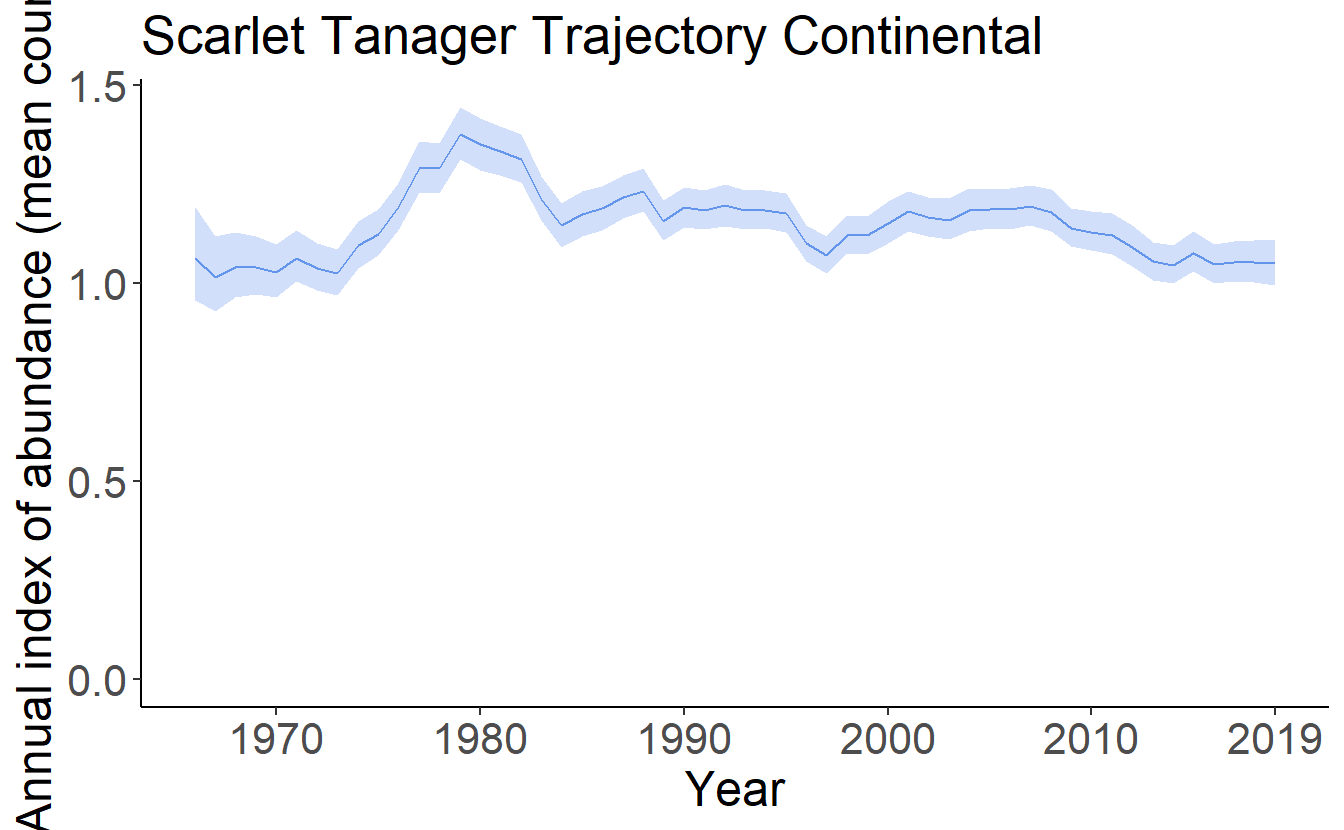
\includegraphics[width=\textwidth]{bbsBayes_Workshop_files/figure-latex/GM2_b-1} \end{center}

\texttt{plot\_indices()} also allows the user to add points to show the observed mean counts as well as stacked dots to indicate the number of observations in each year.

\begin{Shaded}
\begin{Highlighting}[]
\NormalTok{tp2 }\OtherTok{=} \FunctionTok{plot\_indices}\NormalTok{(}\AttributeTok{indices =}\NormalTok{ indices,}
                         \AttributeTok{species =} \FunctionTok{paste}\NormalTok{(}\StringTok{"Scarlet Tanager"}\NormalTok{,}\StringTok{"Full"}\NormalTok{),}
                  \AttributeTok{add\_observed\_means =} \ConstantTok{TRUE}\NormalTok{,}
                  \AttributeTok{add\_number\_routes =} \ConstantTok{TRUE}\NormalTok{)}
\end{Highlighting}
\end{Shaded}

And we can compare these indices plots with those generated using only the smooths.

\begin{Shaded}
\begin{Highlighting}[]
\NormalTok{tp3 }\OtherTok{=} \FunctionTok{plot\_indices}\NormalTok{(}\AttributeTok{indices =}\NormalTok{ indices\_smooth,}
                         \AttributeTok{species =} \FunctionTok{paste}\NormalTok{(}\StringTok{"Scarlet Tanager"}\NormalTok{,}\StringTok{"Smooth"}\NormalTok{),}
                  \AttributeTok{add\_observed\_means =} \ConstantTok{TRUE}\NormalTok{,}
                  \AttributeTok{add\_number\_routes =} \ConstantTok{TRUE}\NormalTok{)}
\end{Highlighting}
\end{Shaded}

Using the patchwork library, we can show these plots side-by-side:

\begin{Shaded}
\begin{Highlighting}[]
\FunctionTok{library}\NormalTok{(patchwork)}
\FunctionTok{print}\NormalTok{(tp2[[}\DecValTok{1}\NormalTok{]]}\SpecialCharTok{+}\NormalTok{tp3[[}\DecValTok{1}\NormalTok{]])}
\end{Highlighting}
\end{Shaded}

\begin{center}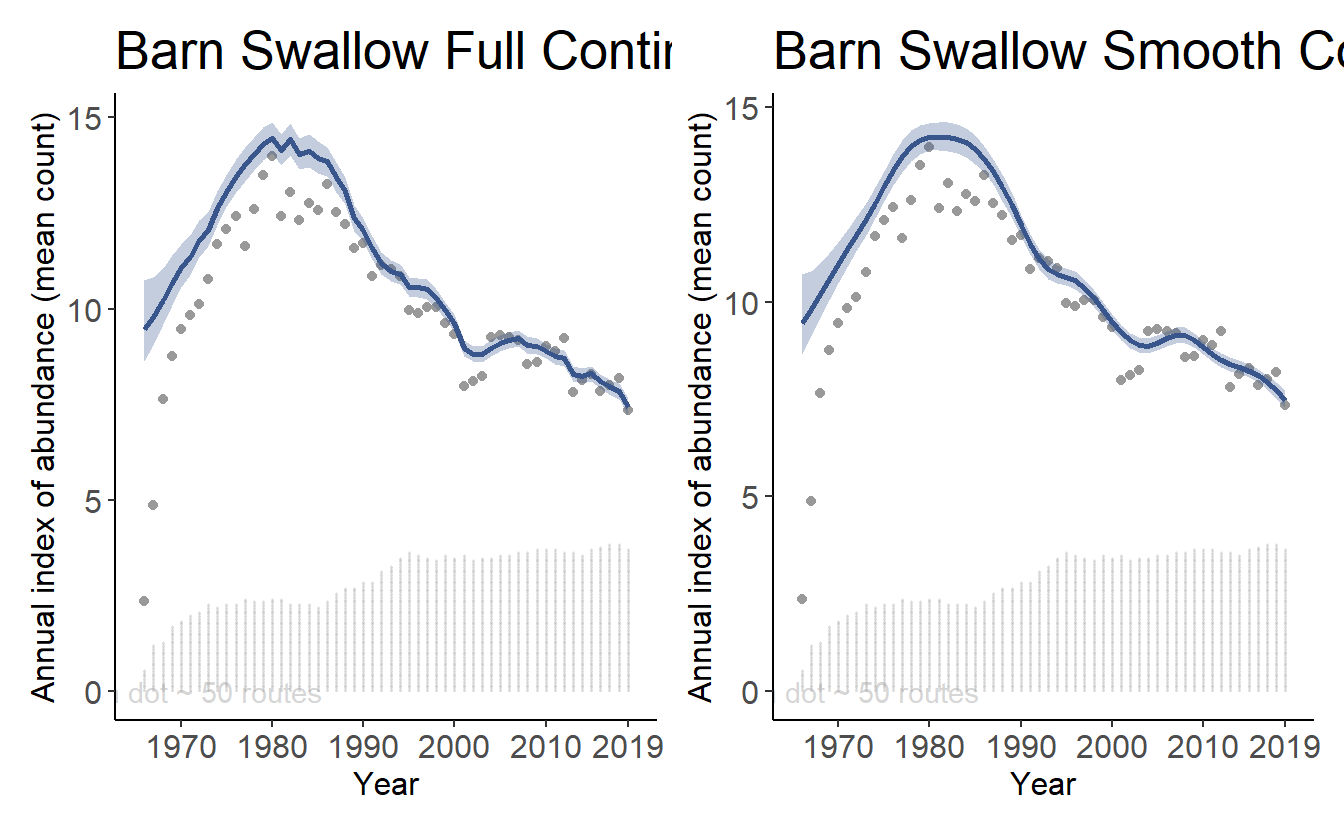
\includegraphics[width=\textwidth]{bbsBayes_Workshop_files/figure-latex/GM5-1} \end{center}

\hypertarget{mapping-the-trends}{%
\section{Mapping the trends}\label{mapping-the-trends}}

The trends can be mapped to produce strata maps coloured by species population trends.

\begin{Shaded}
\begin{Highlighting}[]
\NormalTok{mp }\OtherTok{=} \FunctionTok{generate\_map}\NormalTok{(trends\_smooth,}
                  \AttributeTok{select =} \ConstantTok{TRUE}\NormalTok{,}
                  \AttributeTok{stratify\_by =} \StringTok{"bbs\_cws"}\NormalTok{,}
                  \AttributeTok{species =} \StringTok{"Scarlet Tanager Smooth"}\NormalTok{)}
\FunctionTok{print}\NormalTok{(mp)}
\end{Highlighting}
\end{Shaded}

\begin{center}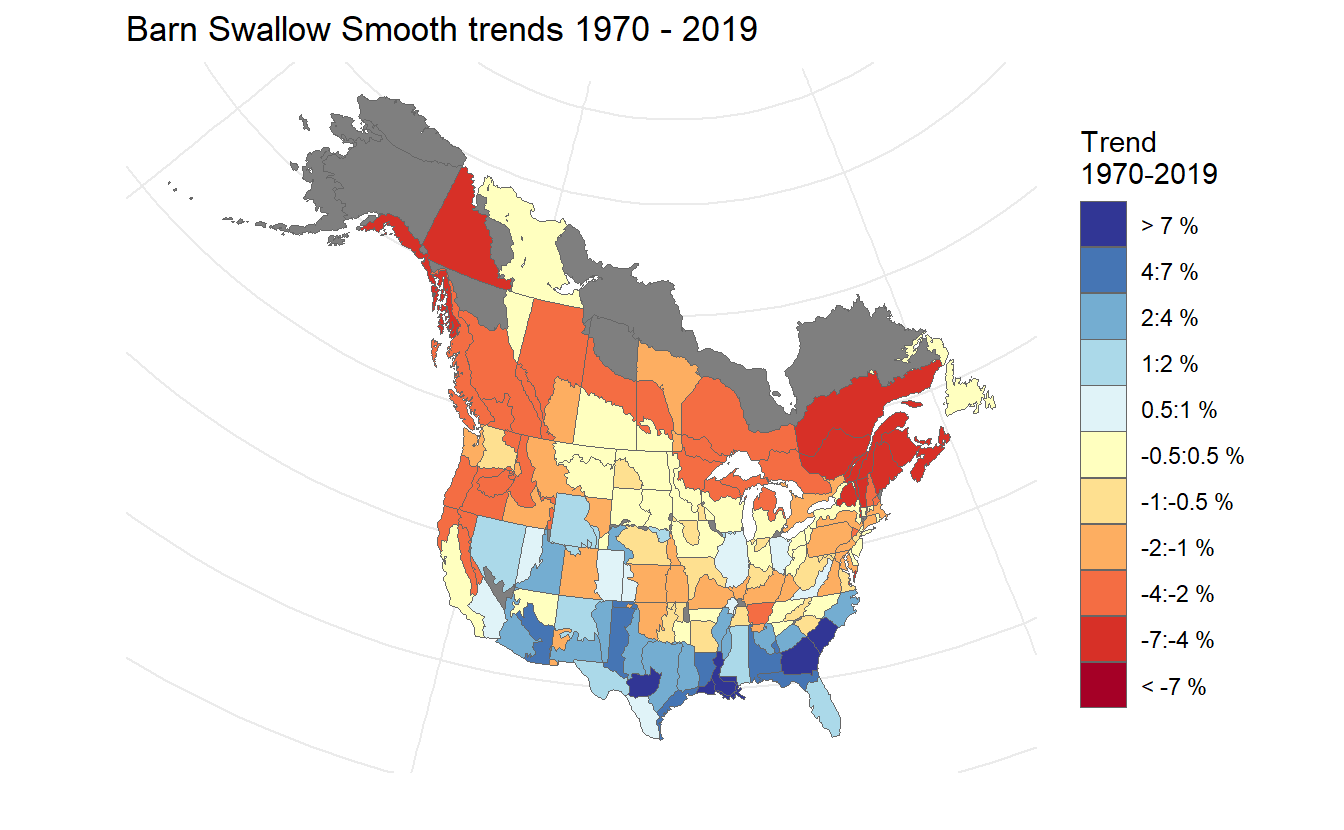
\includegraphics[width=\textwidth]{bbsBayes_Workshop_files/figure-latex/GM6-1} \end{center}

\hypertarget{geofacet-trajectories}{%
\section{Geofacet Trajectories}\label{geofacet-trajectories}}

For stratifications that can be compiled by political regions (i.e., \texttt{bbs\_cws}, \texttt{bbs\_usgs}, or \texttt{state}), the function \texttt{geofacet\_plot} will generate a ggplot object that plots the state and province level population trajectories in facets arranged in an approximately geographic arrangement. These plots offer a concise, range-wide summary of a species' population trajectory.

\begin{Shaded}
\begin{Highlighting}[]
\NormalTok{  gf }\OtherTok{\textless{}{-}} \FunctionTok{geofacet\_plot}\NormalTok{(}\AttributeTok{indices\_list =}\NormalTok{ indices\_smooth,}
                     \AttributeTok{select =} \ConstantTok{TRUE}\NormalTok{,}
                     \AttributeTok{stratify\_by =} \StringTok{"bbs\_cws"}\NormalTok{,}
                     \AttributeTok{multiple =} \ConstantTok{TRUE}\NormalTok{,}
                     \AttributeTok{trends =}\NormalTok{ trends\_smooth,}
                     \AttributeTok{slope =}\NormalTok{ F,}
                     \AttributeTok{species =} \StringTok{"Scarlet Tanager Smooth"}\NormalTok{)}
  
  \FunctionTok{print}\NormalTok{(gf)}
\end{Highlighting}
\end{Shaded}

\begin{center}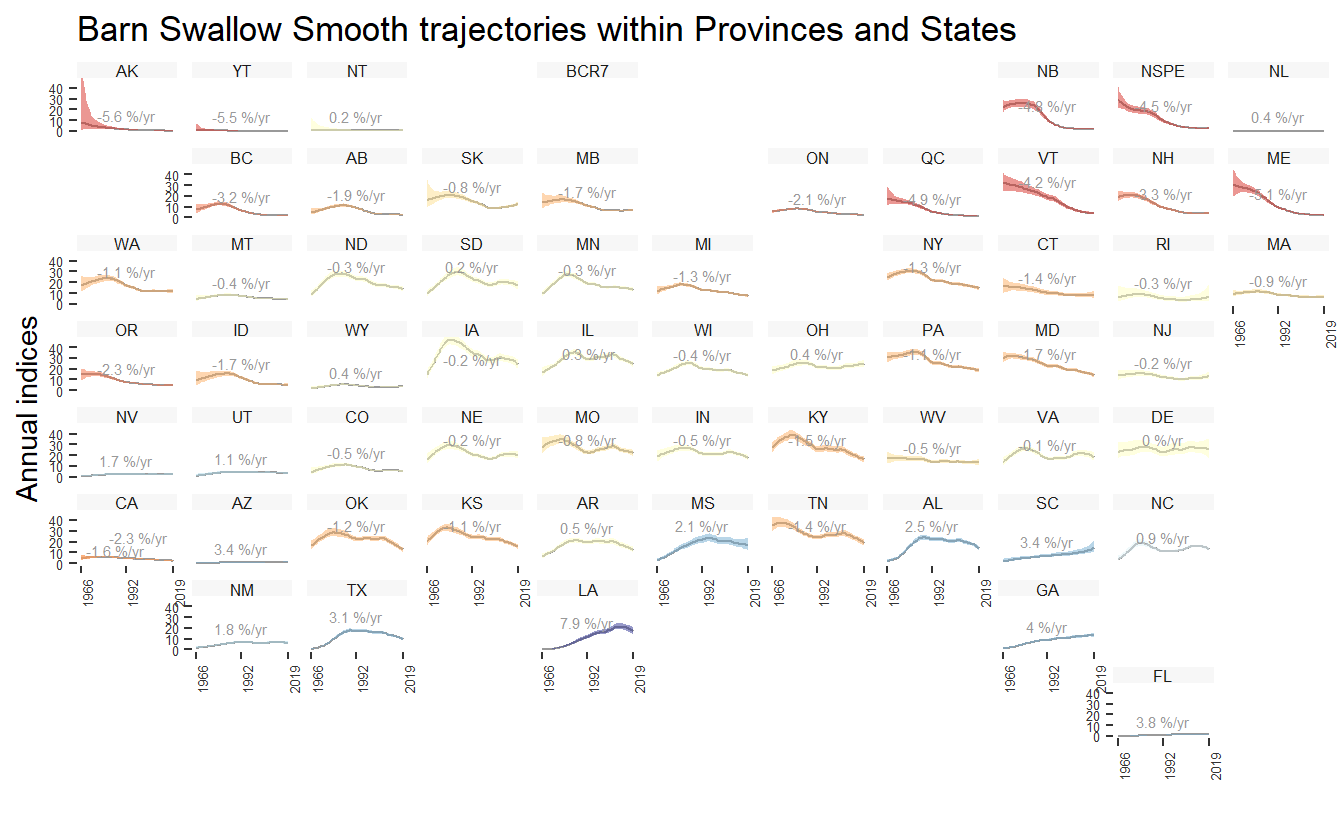
\includegraphics[width=\textwidth]{bbsBayes_Workshop_files/figure-latex/GM7-1} \end{center}

\hypertarget{Adv}{%
\chapter{Advanced options}\label{Adv}}

\hypertarget{custom-regional-summaries}{%
\section{Custom regional summaries}\label{custom-regional-summaries}}

Yes, you can calculate the trend and trajectories for custom combinations of strata, such as a formal trend estimate for populations of Scarlet Tanager in the North East (BCRs 7, 8, 12, 13, and 14).

\begin{Shaded}
\begin{Highlighting}[]
\FunctionTok{load}\NormalTok{(}\StringTok{"jags\_mod\_full.RData"}\NormalTok{) }\CommentTok{\#saved Scarlet Tanager model output and data}
\end{Highlighting}
\end{Shaded}

\hypertarget{define-the-custom-regions-as-a-collection-of-the-existing-strata.}{%
\subsection{Define the custom regions as a collection of the existing strata.}\label{define-the-custom-regions-as-a-collection-of-the-existing-strata.}}

First extract a dataframe that defines the original strata used in the analysis.

\begin{Shaded}
\begin{Highlighting}[]
\NormalTok{st\_comp\_regions }\OtherTok{\textless{}{-}} \FunctionTok{get\_composite\_regions}\NormalTok{(}\AttributeTok{strata\_type =} \StringTok{"bbs\_cws"}\NormalTok{)}
\NormalTok{knitr}\SpecialCharTok{::}\FunctionTok{kable}\NormalTok{(}\FunctionTok{head}\NormalTok{(st\_comp\_regions))}
\end{Highlighting}
\end{Shaded}

\begin{tabular}{l|l|r|l|r|l|l|l}
\hline
prov\_state & region & area\_sq\_km & national & bcr & Province\_State & Country & bcr\_by\_country\\
\hline
AB & CA-AB-10 & 52565 & CA & 10 & Alberta & Canada & Canada-BCR\_10\\
\hline
AB & CA-AB-6 & 445136 & CA & 6 & Alberta & Canada & Canada-BCR\_6\\
\hline
AB & CA-AB-8 & 6987 & CA & 8 & Alberta & Canada & Canada-BCR\_8\\
\hline
AB & CA-AB-11 & 149352 & CA & 11 & Alberta & Canada & Canada-BCR\_11\\
\hline
AK & US-AK-1 & 9551 & US & 1 & ALASKA & United States of America & United States of America-BCR\_1\\
\hline
AK & US-AK-2 & 283405 & US & 2 & ALASKA & United States of America & United States of America-BCR\_2\\
\hline
\end{tabular}

Then add a column to the dataframe that groups the original strata into the desired custom regions.

\begin{Shaded}
\begin{Highlighting}[]
\NormalTok{st\_comp\_regions}\SpecialCharTok{$}\NormalTok{NorthEast }\OtherTok{\textless{}{-}} \FunctionTok{ifelse}\NormalTok{(st\_comp\_regions}\SpecialCharTok{$}\NormalTok{bcr }\SpecialCharTok{\%in\%} \FunctionTok{c}\NormalTok{(}\DecValTok{7}\NormalTok{,}\DecValTok{8}\NormalTok{,}\DecValTok{12}\SpecialCharTok{:}\DecValTok{14}\NormalTok{),}\StringTok{"NorthEast"}\NormalTok{,}\StringTok{"Other"}\NormalTok{)}
\end{Highlighting}
\end{Shaded}

\hypertarget{use-defined-regions-to-estimate-indices-and-trends}{%
\subsection{Use defined regions to estimate indices and trends}\label{use-defined-regions-to-estimate-indices-and-trends}}

st\_comp\_regions can now be used as the dataframe input to the argument alt\_region\_names in \texttt{generate\_indices()}, with ``NorthEast'' as the value for the argument regions. The relevant trends can be calculated using just the \texttt{generate\_trends()} function.

\begin{Shaded}
\begin{Highlighting}[]
\FunctionTok{library}\NormalTok{(patchwork)}
\NormalTok{custom\_indices }\OtherTok{\textless{}{-}} \FunctionTok{generate\_indices}\NormalTok{(}\AttributeTok{jags\_mod =}\NormalTok{ jags\_mod,}
                                      \AttributeTok{jags\_data =}\NormalTok{ jags\_data,}
                                      \AttributeTok{alt\_region\_names =}\NormalTok{ st\_comp\_regions,}
                                      \AttributeTok{regions =} \StringTok{"NorthEast"}\NormalTok{)}
\NormalTok{tp }\OtherTok{=} \FunctionTok{plot\_indices}\NormalTok{(}\AttributeTok{indices =}\NormalTok{ custom\_indices,}
                         \AttributeTok{species =} \StringTok{"Scarlet Tanager"}\NormalTok{,}
                  \AttributeTok{add\_observed\_means =} \ConstantTok{TRUE}\NormalTok{,}
                  \AttributeTok{add\_number\_routes =} \ConstantTok{TRUE}\NormalTok{)}
\end{Highlighting}
\end{Shaded}

\begin{Shaded}
\begin{Highlighting}[]
\FunctionTok{print}\NormalTok{(tp[[}\DecValTok{1}\NormalTok{]])}
\FunctionTok{print}\NormalTok{(tp[[}\DecValTok{2}\NormalTok{]])}
\end{Highlighting}
\end{Shaded}

\begin{center}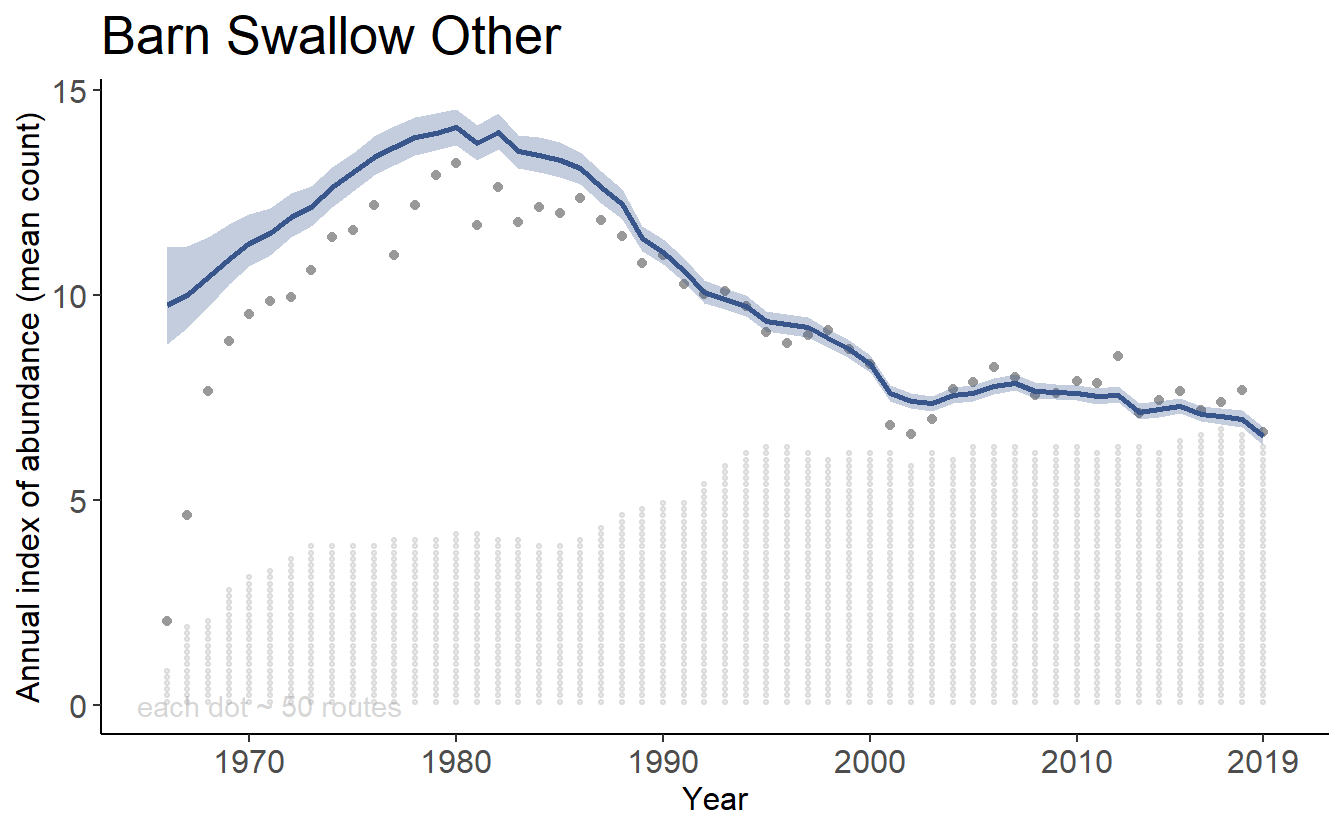
\includegraphics[width=\textwidth]{bbsBayes_Workshop_files/figure-latex/A5plot-1} 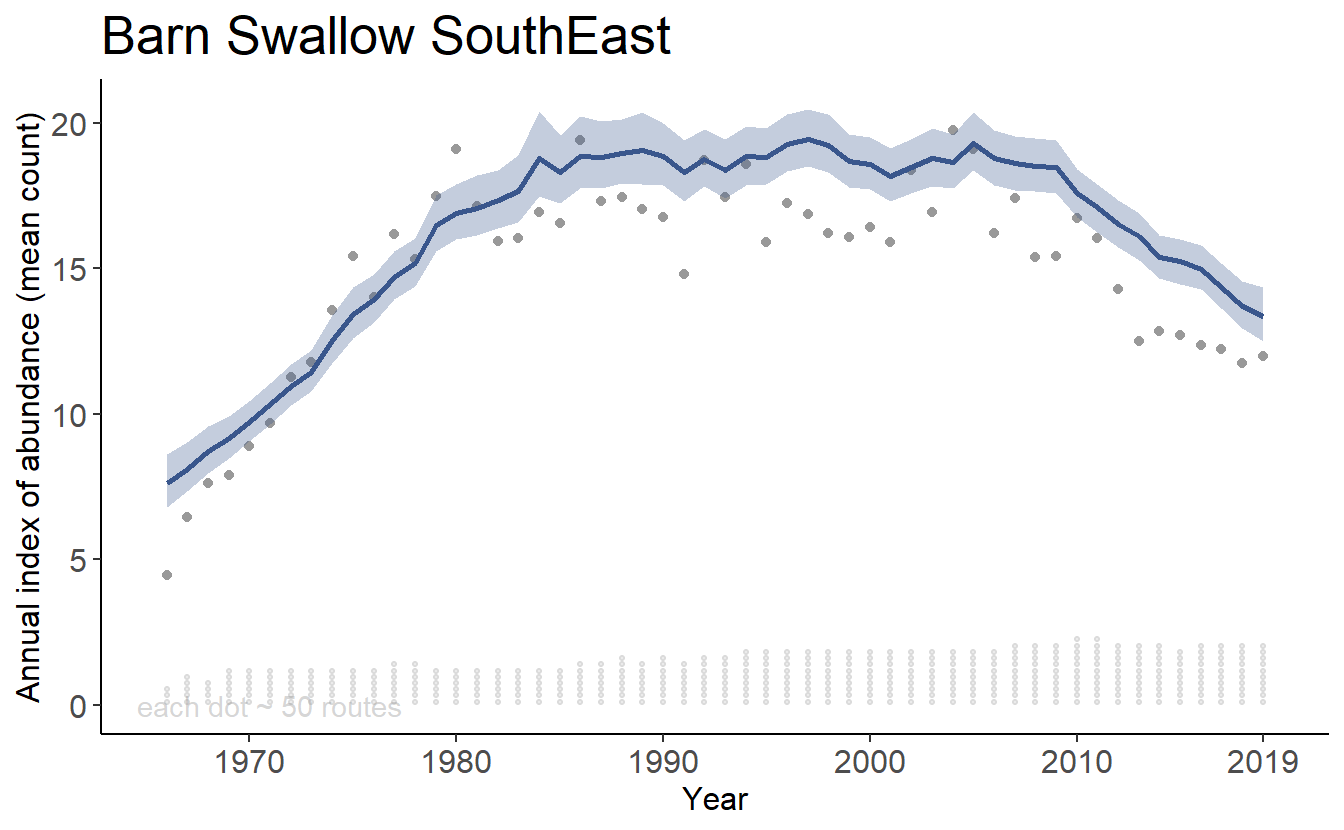
\includegraphics[width=\textwidth]{bbsBayes_Workshop_files/figure-latex/A5plot-2} \end{center}

Calculate trends

\begin{Shaded}
\begin{Highlighting}[]
\NormalTok{custom\_trends }\OtherTok{\textless{}{-}} \FunctionTok{generate\_trends}\NormalTok{(}\AttributeTok{indices =}\NormalTok{ custom\_indices)}
\NormalTok{knitr}\SpecialCharTok{::}\FunctionTok{kable}\NormalTok{(custom\_trends[,}\FunctionTok{c}\NormalTok{(}\DecValTok{1}\NormalTok{,}\DecValTok{3}\NormalTok{,}\DecValTok{8}\NormalTok{,}\DecValTok{9}\NormalTok{,}\DecValTok{14}\NormalTok{)])}
\end{Highlighting}
\end{Shaded}

\hypertarget{exporting-the-jags-model}{%
\section{Exporting the JAGS model}\label{exporting-the-jags-model}}

You can easily export any of the bbsBayes models to a text file.

\begin{Shaded}
\begin{Highlighting}[]
\FunctionTok{model\_to\_file}\NormalTok{(}\AttributeTok{model =} \StringTok{"slope"}\NormalTok{,}
              \AttributeTok{filename =} \StringTok{"my\_slope\_model.txt"}\NormalTok{)}
\end{Highlighting}
\end{Shaded}

Then, you can modify the model text (e.g., try a different prior) and run the modified model

\begin{Shaded}
\begin{Highlighting}[]
\NormalTok{run\_model }\OtherTok{\textless{}{-}} \ControlFlowTok{function}\NormalTok{(... ,}
                      \AttributeTok{model\_file\_path =} \StringTok{"my\_modified\_slope\_model.txt"}\NormalTok{,}
\NormalTok{                      ... )}
\end{Highlighting}
\end{Shaded}

Details coming soon\ldots{}

\hypertarget{customizing-the-jags-model-and-data}{%
\section{Customizing the JAGS model and data}\label{customizing-the-jags-model-and-data}}

You can even export the bbsBayes model as text, and modify it to add in covariates. For example a GAM smooth to estimate the effect of the day of year on the observations, or an annual weather covariate, or\ldots{} Then add the relevant covariate data to the jags\_data object, and you're off! We'll add some more details and examples soon.

\hypertarget{comparing-models}{%
\section{Comparing Models}\label{comparing-models}}

Finally, bbsBayes can be used to run Bayesian cross-validations. For example, the \texttt{get\_final\_values()} function is useful to provide an efficient starting point for a cross-validation runs, without having to wait for another full burn-in period.

Paper that includes an example of how to implement a cross-validation using bbsBayes.

Pre-print: \url{https://doi.org/10.1101/2020.03.26.010215}
Supplement: \url{https://zenodo.org/badge/latestdoi/228419725}

NOTE: although bbsBayes includes functions to calculate WAIC, recent work has shown that WAIC performs very poorly with the BBS data (\url{https://doi.org/10.1650/CONDOR-17-1.1}). We recommend a k-fold cross-validation approach, as in the above zenodo archive.

\hypertarget{Ref}{%
\chapter{References}\label{Ref}}

\hypertarget{refs}{}
\begin{CSLReferences}{1}{0}
\leavevmode\hypertarget{ref-link2002}{}%
Link, William A., and John R. Sauer. 2002a. {``A Hierarchical Analysis of Population Change with Application to Cerulean Warblers.''} \emph{Ecology} 83 (10): 2832--40. \url{https://doi.org/10.1890/0012-9658(2002)083\%5B2832:AHAOPC\%5D2.0.CO;2}.

\leavevmode\hypertarget{ref-link2002a}{}%
---------. 2002b. {``A Hierarchical Analysis of Population Change with Application to Cerulean Warblers.''} \emph{Ecology} 83 (10): 2832--40. \url{https://doi.org/10.1890/0012-9658(2002)083\%5B2832:AHAOPC\%5D2.0.CO;2}.

\leavevmode\hypertarget{ref-link}{}%
Link, William A., John R. Sauer, and Daniel K. Niven. n.d. {``Model Selection for the North American Breeding Bird Survey.''} \emph{Ecological Applications} n/a (n/a). \url{https://doi.org/10.1002/eap.2137}.

\leavevmode\hypertarget{ref-sauer2011}{}%
Sauer, John R., and William A. Link. 2011. {``Analysis of the North American Breeding Bird Survey Using Hierarchical Models.''} \emph{The Auk} 128 (1): 87--98. \url{https://doi.org/10.1525/auk.2010.09220}.

\leavevmode\hypertarget{ref-smith2020a}{}%
Smith, Adam C., and Brandon P.M. Edwards. 2020. {``North American Breeding Bird Survey Status and Trend Estimates to Inform a Wide-Range of Conservation Needs, Using a Flexible Bayesian Hierarchical Generalized Additive Model.''} \url{https://doi.org/10.1101/2020.03.26.010215}.

\leavevmode\hypertarget{ref-smith2014}{}%
Smith, Adam C., Marie-Anne R. Hudson, Constance Downes, and Charles M. Francis. 2014. {``Estimating Breeding Bird Survey Trends and Annual Indices for Canada: How Do the New Hierarchical Bayesian Estimates Differ from Previous Estimates?''} \emph{The Canadian Field-Naturalist} 128 (2): 119. \url{https://doi.org/10.22621/cfn.v128i2.1565}.

\end{CSLReferences}

\end{document}
